\RequirePackage{ifpdf}
\documentclass[a4paper,11pt,openany]{kth-mag}
%\let\ifpdf\relax
\usepackage[T1]{fontenc}
\usepackage{textcomp}
\usepackage{lmodern}
\usepackage[latin1]{inputenc}
\usepackage[swedish,english]{babel}
\usepackage{modifications}
\usepackage{graphicx}
\usepackage{amsmath}
\usepackage{times}
\usepackage{subfigure}
\usepackage{multirow}
\usepackage{colortbl,booktabs}


\title{Prediction of peptide retention time based on Gaussian Process}


\foreigntitle{}
\author{XuanBin Qiu}
\date{March 2015}
\blurb{Master's Thesis at NADA\\
External Supervisor: Lukas K\"{a}ll\\
Internal Supervisor: Patric Jensfelt\\
Examiner: Stefan Carlsson}
\trita{TRITA 2015-3-19}

\begin{document}
\frontmatter
\pagestyle{headings}
\removepagenumbers
\maketitle
\selectlanguage{english}
\begin{abstract}
  Retention time (RT) as an important evidence can be used to analysis the peptide 's  properties. Because of the nonlinear concentration curve of the whole range of run time and the interactions among peptides, the retention time prediction of peptide has low accuracy,
  and thus is less effective in the validation of peptide identifications. Besides, the large amount of time on generating features also need to be reduced. This thesis presents a alterative machine learning methods to predict the retention time of a set of peptide in hand. In order to address the precision and computational cost problem, we introduce Gaussian Process as the trained model and use a new feature extracted method called BOW to generate the features for training the model. We also investigate the effect in terms of kernel function and their parameters. The results show high precision of the prediction and relatively low time cost.
\end{abstract}

\clearpage
\tableofcontents*

\mainmatter
\pagestyle{newchap}
\chapter{Introduction}
\fontsize{12pt}{16pt}\selectfont
\section{Background}
Protein, the most essential component of all the cells and organisms, plays an irreplaceable role in people's daily lives including providing energy, strengthen immune system and catalyzing metabolic reactions within the body. Therefore, the study of the properties of protein is very necessary and considered as one of most important subject in biological field.\\

\noindent
Before introducing the background, we will briefly describe a few concepts that we will involve later so that one could understand the method easier.
\begin{itemize}
  \item Liquid Chromatography: A technique in analytic chemistry used to separate the components in a mixture, to identify each component, and to quantify each component.
  \item Peptide: Short sequence(chain) of amino acid connected by peptide bonds as Fig. \ref{fig:Fig3} It's distinguished from proteins on the basis of size which only contain approximately 50 or fewer amino acid.
\begin{figure}[h!]
  \centering
  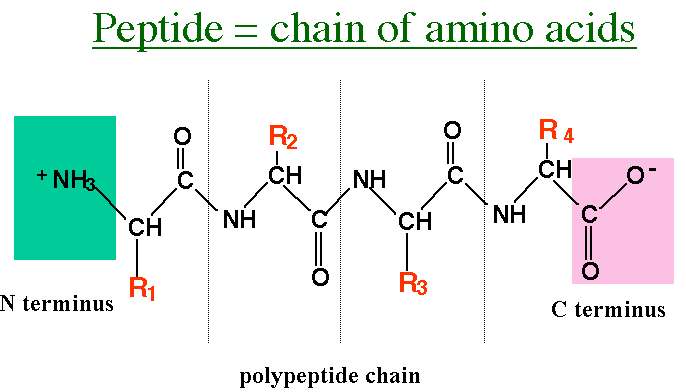
\includegraphics[width=6cm]{./peptide.png}\\
  \caption{Peptide model}\label{fig:Fig3}
\end{figure}
  \item Amino acid: Biologically important organic compounds composed of amine (-NH2) and carboxylic acid (-COOH) functional groups, along with a side-chain specific to each amino acid. There are approximately 20 basic types and Fig. \ref{fig:Fig4} is an example of one of them. They are the basic unit composed of protein, giving protein their specific structural form so that they could have biological activity.
\begin{figure}
  \centering
  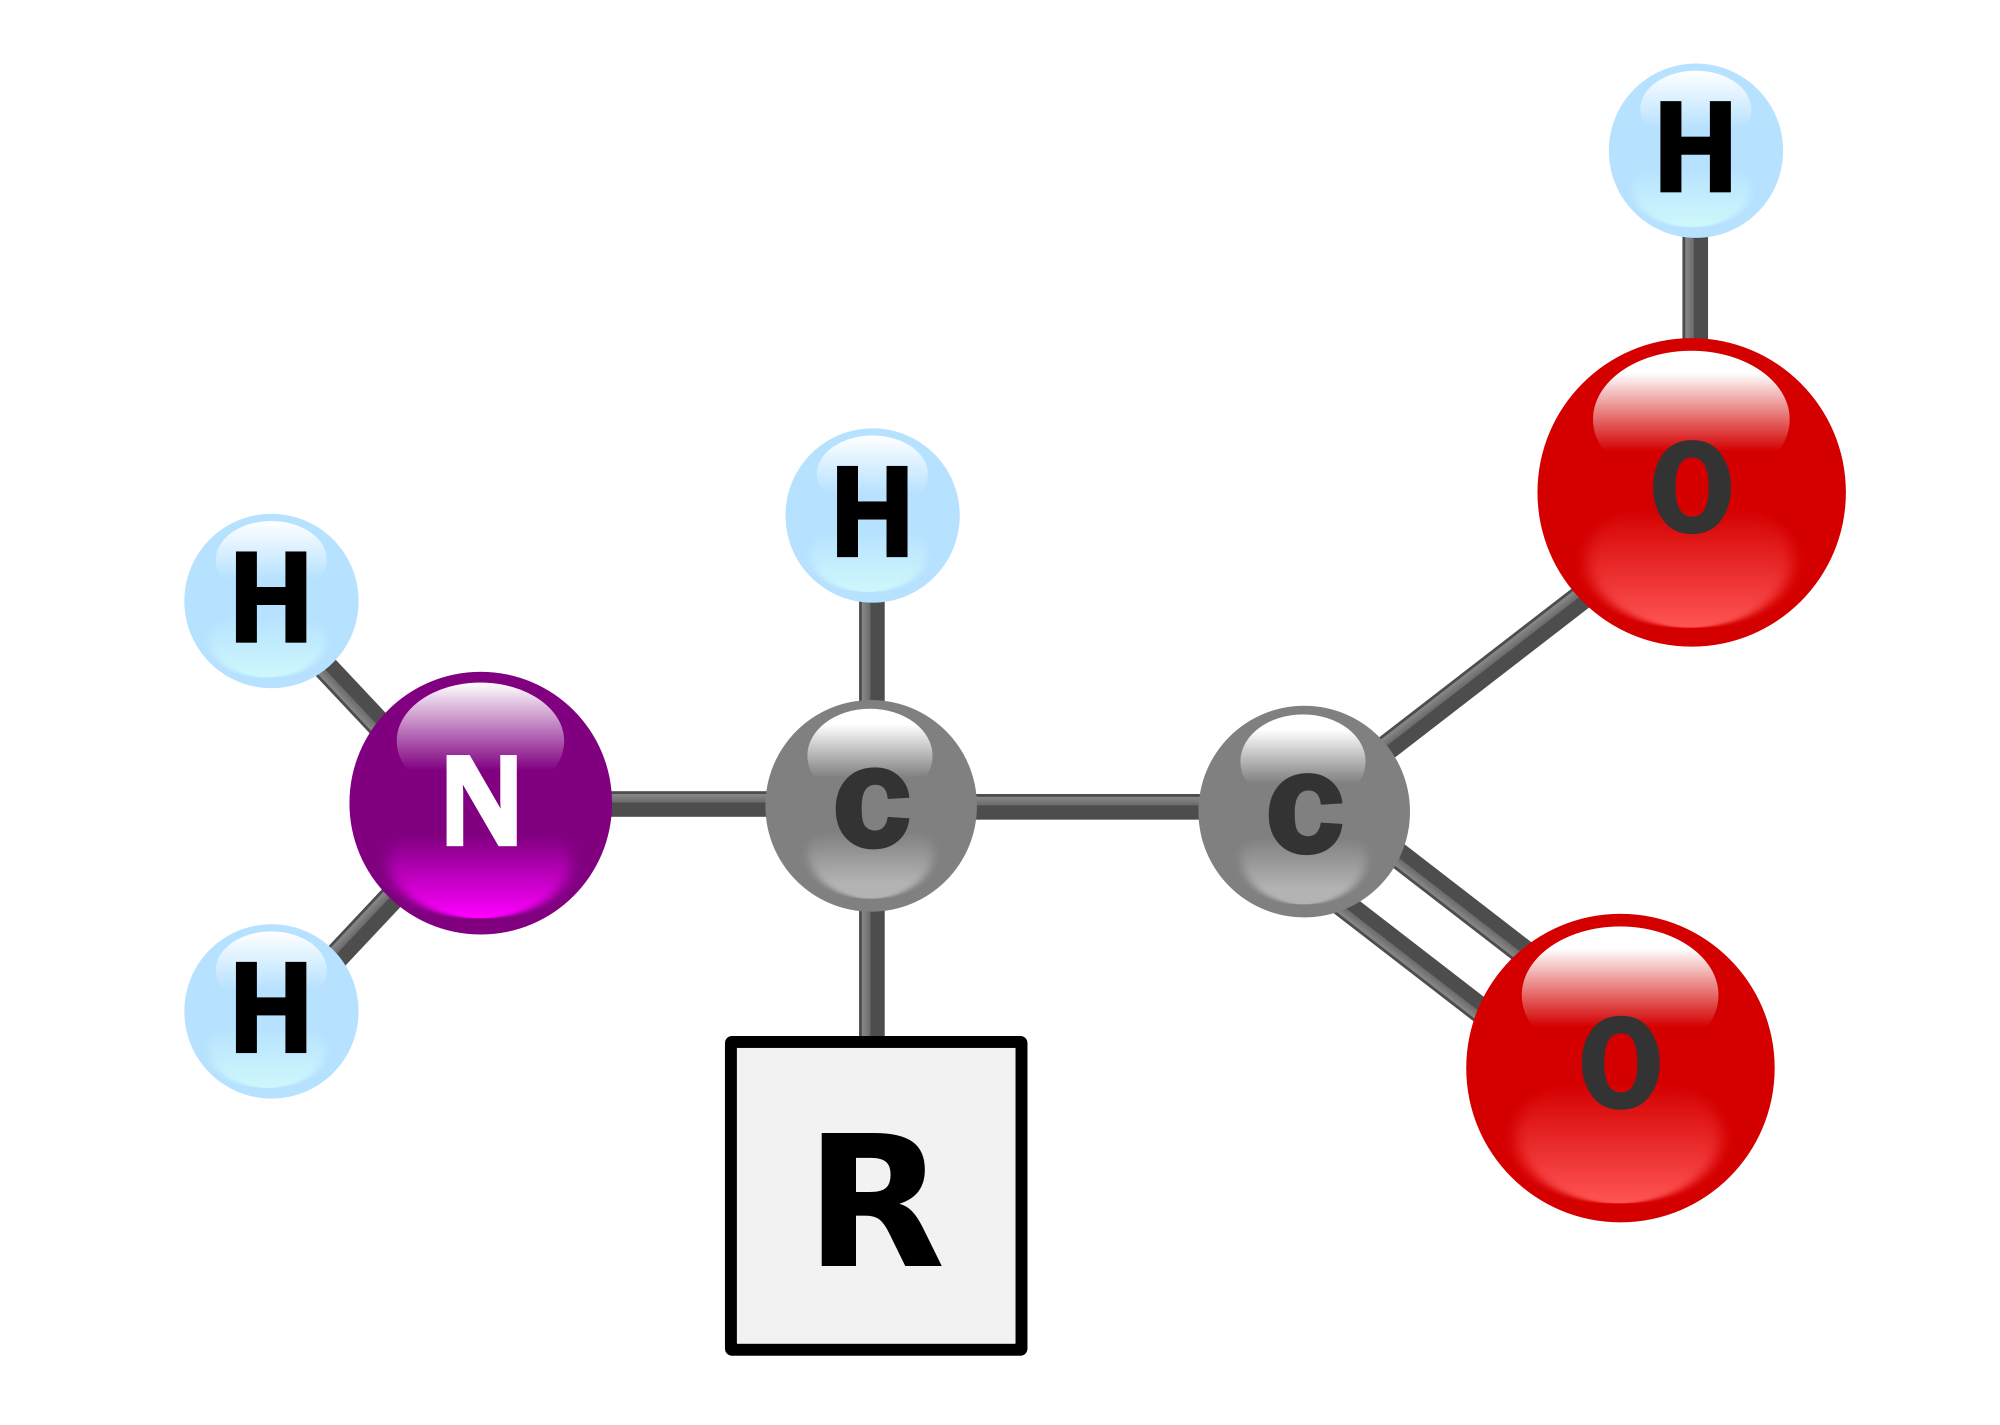
\includegraphics[width=6cm]{Alpha_AminoAcidball.png}\\
  \caption{Alpha Amino Acid}\label{fig:Fig4}
\end{figure}
  \item Hydrophobicity: A physical property of a molecule that is seemingly repelled from a mass of water. It has a great impact in terms of interaction between different proteins, the structure of the protein. And more importantly, in this case, the peptide retention time has a strong relationship with it.
\end{itemize}

\noindent
To analyze the protein content, one of most popular technique is Mass spectrometry\\(MS) based method. This technique has three main steps, firstly, the protein in the mixture of interest will be broken into peptide. Then the resulting  peptides are separated according to their hydrophobicity on a liquid chromatography(LC) column. In the end, those peptide will eluted from the column and ionized by electrospray ionization. The results are a set of spectra which contain the valuable  information about the proteins in the sample.\\

\noindent
Among these three steps, the most important one is the peptide separation in the column. Retention time(RT) is the amount of time that a peptide needs to go through the column. It is a useful feature in many aspects. It may be used in experiments involving chemometric analyses of peptide mixtures. What's more, it provides us a new perspective to investigate the behavior and biological characters of the protein. An extensive amount of research has been conducted into predicting peptide retention times. The Sequence Specific Retention Calculator(SSRC) which predicts retention times based on amino acid sequences is available on-line. The main algorithm behind those applications is mostly based on either Support Vector Regression(SVR) or Artificial Neural Network(ANN). \\

\section{Problem Statement}
\noindent
All of these methods have their own drawbacks and still needs to be improved. One alternative option is to implement the Gaussian Process(GPs) to build the predictive model. GPs provides a flexible framework for probabilistic regression and is widely used to solve the high-dimensional, small-sample or nonlinear problems. It seems that the properties of GPs can overcome the shortages of ANN and SVR. Yet none of the existing publications has the prediction of retention times for peptides analyzed with the use of Gaussian Process.\\

\noindent
Therefore, the top priority of this thesis is to develop a Gaussian Process Regression model in terms of predicting the peptide retention time and investigate the performance of it before optimization and after optimization of its parameters.\\

\noindent
Besides, this thesis will also strive to find some features with less biological meaning to represent the peptide for training model and compare their performance to the biological features.\\



\section{Outline}
\noindent
The structure of the paper is as follows, we will first introduce the related work of retention time prediction that have already been done by the others in section 2. It will be followed by the detailed description of Gaussian Process in section 3. The theory behind Gaussian Process and detailed mathematics derivation will also be covered in this section. Section 4 introduces three different methods regarding features selections of Gaussian Process. The optimization will be covered in section 5 and two different method will be used to optimize the parameters in the previous model. Then, the experimental results and evaluation will be analyzed in section 6. Finally, we will discuss the future work and give some perspectives for it in section 7.



\chapter{Related Work}
\fontsize{12pt}{16pt}\selectfont
\noindent
Prediction of the retention time for a given peptide could help to improve the confidence of peptide identifications. Therefore, developing efficient algorithms and establish proper model to generate the prediction of peptide has become more important and necessary.\\

\noindent
However, to make the prediction successfully, there are two problems needed to be considered. Firstly, what kind of model will have better performance of the prediction. Secondly, what factors will have an great impact on the retention time. Unfortunately, both of these two questions remain unclear so far. Therefore, in order to solve the questions, a number of models based on different features have been proposed to characterize quantitatively the peptide and to predict its retention time.\\

\section{Models / Methods}
\noindent
There are different kinds of machine-learned models that have been implemented. One of the model is multiple linear regression(MLR) model. This model was implemented by Baczek T, Wiczling P, Marszall M, et al of \cite{foo1} to predict the peptide retention time at different HPLC conditions and shows high precision. However,the linear regression model mainly depends on the chromatographic condition and thus prediction bias could be a serious problem when the model is used under different circumstance. \\

\noindent
Another model is the artificial neural network(ANN) proposed by Petritis K et al. in \cite{foo2}. The ANN model was based on the contributions of individual amino acids taken the neighborhood effect into account and a data set of 7000 was used for the training. The large amount of experimental data provided by this approach produced high accuracy of the retention time prediction and enhance the confidence of the peptide identification. In addition, the initial ANN model has been improved later in 2006. In \cite{foo3}, Petritis K, Kangas LJ, Yan B, et al have improved the ANN model by adding more descriptors, such as peptide length, sequence, hydrophobicity as well as nearest-neighbor amino acid. Each of the peptide is characterized by 1052 features instead of 20. The new model was trained by 345,000 peptide and tested using another 1303 confidently identified peptide which reported excellent performance.\\

\noindent
Although a great deal of effort has been made to improve the model, there are still some remained issues. One of the main weaknesses of this model is its time consumption. In order to train this model, a large amount of training data is required which will result in a high cost in terms of both time and resources. What's worse, its high computational cost also implies its weakness in terms of repeatability and comparability which are essential to laboratory research. It also limited its development for commercial purpose.\\

\noindent
In order to solve this problem, another alternative machine-learned method support vector machine(SVMs) has been implemented. Klammer et al. in \cite{foo4} proposed a predictor based on this method. SVMs requires fewer data to train the model than ANNs and reduce the computational cost dramatically. Besides, dynamic SVR model avoids the RT variation between different chromatographic conditions which could have better performance than the linear regression model in terms of adaptability. However, using small dataset with low complexity to train the model also leads to the poor performance in terms of accurate regression and gives lower quality prediction compared to the ANNs.\\


\noindent
To enhance the capacity of the predictor and raise the predicted accuracy, Luminita Moruz in \cite{foo5} has developed a new predictor, ELUDE,  based on support vector regression (SVR). The predictor firstly derives a retention time index for the condition at hand. Then by using those indices, the predictor creates 60 peptide features which are optimally combined during a second training procedure. After that, $\epsilon-SVR$, a popular kind of SVR model, is used to train the model based on the features. The resulting retention model can be subsequently used to predict the retention time of other peptides of interest. \\

\noindent
The performance of Elude is excellent and considered as one of the state-of-the-art retention time predictors. However, one of the shortcomings of the Elude algorithm is the rather limited use of positional information. The retention index trained in-house on which many of the other features are based is calculated using only the amino acid composition. Adding positional data is likely to capture more information, and thus lead to higher prediction accuracies \cite{foo6}.\\

\noindent
However, even with the proper models, the prediction could fail or the precision could be extremely low if the selected features are improper or unrepresentative. So the features selection is also an essential part of an successful prediction.\\

\section{Features}
\noindent
The effect of individual amino acid was firstly taken into account when building the model because evidences implied that the inclusion of this type of additional information could increase the confidence of protein identification of the peptide \cite{foo1} and the chromatographic behavior of a peptide is mainly dependent on its amino acid composition \cite{foo7}. A set of retention time coefficients were generated from only different amino-acid composition by using iterative regression methods.\cite{foo8} \cite{foo9} \cite{foo10}\\

\noindent
However, the author of \cite{foo9} pointed out that the relative location of different amino acid in a peptide could affect the behavior of the peptide too. The author of \cite{foo11} has also emphasized the relation between the chromatographic behavior of peptides and their amino acid composition. It is for sure that different values of retention coefficients of the same amino acid need to be assigned according to different peptides and different neighborhoods. Besides, the other biological characters, such as hydrophobicity \cite{foo12}, ion-pairing reagents \cite{foo13}, stationary phase \cite{foo14} and even the length of the peptide could influence the peptide retention behavior. \\

\noindent
Thus, in \cite{foo15}, O.V. Krokhin, R. Craig have developed an improved model, Sequence-Specific Retention Calculator(SSRC), for prediction of retention times in ion pair reversed-phase based on a database of 346 peptides. The ability of this model for prediction can assist detailed peptide mapping significantly, thus increase confidence in peptide identification and the protein characterization. However, the model is not completed and has not included amino acid modification that may occur during the sample preparation. In addition, the prediction capacity becomes worse for experimental condition which is diverging from the setup.\\

\noindent
After SSRC, there are several different kinds of factors have been used. One of them is the structural descriptors. The author has employed the Quantitative structure-retention relationships with the information of the peptide's chemical characters and its structure in article \cite{foo16}. The predictor implemented in article \cite{foo1} is also based on three types of chemical structural descriptors and both of them showed good results with the experimental data.\\

\noindent
In general, most of the features that are widely used now have strong biological meaning, such as amino acid composition, hydrophobicity of the peptide and some other chemical structural descriptors and the performances of these features can fulfill the requirement. However, these features are mostly limited within the biological field and few of the less-biological meaning features have been tried so far.\\

\noindent
From the perspective of computer science, anything that can represent an object could be considered as a feature of this object. Therefore, it is worth to believe that some less-biological meaning features could give the same performance in this case. In this thesis,  some features with less biological meaning will be utilized and their performance will be compared to the traditional biological features.


\chapter{Gaussian Process}
\fontsize{12pt}{16pt}\selectfont

Gaussian Process is an supervised machine learning method based on the context of Bayesian theory and statistical learning. In order to understand the theory behind and build a appropriate Gaussian Process model, this chapter starts with a brief introduction of the supervised learning method as well as the specification of Standard Bayesian linear Regression. Then we will specify the Gaussian Process in our case along with the detailed mathematical derivation. After that, we will specify the concept of multi-kernel functions in Gaussian Process and explain the properties of it. Finally, we will make a comparison between Gaussian Process and the other two methods: ANNs and SVR so that we could see the strengths of Gaussian Process.

\section{Standard Bayesian linear Regression}

Let's first consider a set of input $x = \{(x_{i},y_{i}) | i =1,2...n\}$ along with some noise $\epsilon$. In the regression setting, the targets are real values but the observations are with additive noise. We are interested in inferring the relationship between inputs and targets, i.e. the conditional distribution of the targets given the inputs.\\

\noindent
In supervised learning, one way to decide this relationship is using parametric regression which is determine a set of $w$ as the best descriptors of the model between the inputs and outputs. Now, the problem comes to how to define if the model is good enough.\\

\noindent
To solve this problem, two possible methods have been carried out. Loss Function Method and Maximum Likelihood Method. The first one is achieved by optimizing the parameters $w$ that minimizing the predefined loss function, such as minimal squared error function(MSE). However, one of the obvious shortages of this method is the over-fitting. To minimize the error of the model, one would increase the complexity of the model that might easily result in the over-fitting problem. Even though the precision of model in terms of training data could be high enough, its predictive capacity for unknown data could be really bad and unacceptable. In addition, making a simpler model by ignoring the noise could avoid the over-fitting problem but could also lead to lower accuracy for prediction.\\

\noindent
An alternative way to identify the quality of model is Maximum Likelihood, also known as Bayesian regression. The idea of this method is replacing the loss function by the jointly probability distribution with predefined noise (Likelihood function) and search for the parameters $w$ that maximize the likelihood function to build the model.\\

\noindent
Let's consider the dataset $x = \{(x_{i},y_{i}) | i =1,2...n\}$ mentioned before as the input. The Bayesian analysis of the linear regression model can be written as :
\begin{equation} \label{eq:2}
f_{x}=x^{T}w, \quad  y = f_{x}+\epsilon ,
\end{equation}

\noindent
where $x$ is the input vector, $w$ is the parameters(weights) of the input for the linear model. The function value is represented by $ f_{x}$ and an bias (noise) is included. We assume that the $\epsilon$ is the independent identically distributed Gaussian noise with the zero mean and variance $\sigma_{n} ^{2}$.
\begin{equation} \label{eq:3}
\epsilon \sim N(0, \sigma_{n} ^{2}) ,
\end{equation}

\noindent
The likelihood function, the probability density of the observation given the parameters, will then have the following form:
\begin{equation} \label{eq:4}
p(y|x,w) = \prod_{i=1}^{n}p(y_{i}|x_{i},w) = \prod_{i=1}^{n}\frac{1}{\sqrt{2\pi}\sigma_{n}}exp(-\frac{(y_{i}-x_{i}^{T}w)^{2}}{2\sigma_{n}^{2}})
\end{equation}

\noindent
The idea of Bayesian linear model is mainly based on the posterior distribution computed by Bayes' rule:
\begin{equation} \label{eq:5}
p(w|y,x) = \frac{p(y|x,w)p(w)}{p(y|x)}
\end{equation}

\noindent
To calculate the posterior, we also need a prior over the parameters. The prior is usually considered as to represent our prior beliefs over the distribution of the parameters we expect to observe before seeing any data. Therefore, we put a zero mean Gaussian prior with covariance matrix $\Sigma$ on the weights:
\begin{equation} \label{eq:6}
w \sim N(0,\Sigma)
\end{equation}

\noindent
Another essential part is the marginal likelihood function $p(y|x)$. The marginal likelihood,(normalizing constant), gives the likelihood of the output by considering only one specific kind of input and is independent of the other factors. To be specific, the marginal likelihood of expected output here only consider the effect of the input $x$ without taking the effect of the weights $w$ into account. Therefore, it is given by
\begin{equation} \label{eq:7}
p(y|x) = \int p(y|x,w)p(w)dw
\end{equation}

\noindent
By now, combine the likelihood function in \ref{eq:4} with the prior in \ref{eq:6} and marginal likelihood function in \ref{eq:7}, we could obtain the actual form of the posterior $p(w|x,y)$ in \ref{eq:5}
\begin{equation} \label{eq:8}
p(w|y,x) = \frac{p(y|x,w)p(w)}{p(y|x)} \sim exp(-\frac{1}{2}(w-\bar w)^{T}(\frac{1}{\sigma_{n}^{2}}xx^{T}+\Sigma^{-1})(w-\bar w))
\end{equation}

\noindent
From \ref{eq:8}, it can be seen that the posterior is actually another Gaussian distribution with the new mean and new covariance matrix.\\
\begin{align}\label{eq.9}
    &\bar w= \sigma_{n}^{-2}(\frac{1}{\sigma_{n}^{2}}xx^{T}+\Sigma^{-1})^{-1}xy\notag \\
    &\Sigma_{new} = \frac{1}{\sigma_{n}^{2}}xx^{T}+\Sigma^{-1}
\end{align}

\noindent
For Bayesian linear regression, the prediction is made by all possible parameters along with corresponding posterior probability. Thus, we could conclude the predictive jointly distribution of the output $f_{new}$ of an new data point $x_{new}$ based on the training dataset $x$ along with their weights $w$ and their outputs $y$ as follows :
\begin{align} \label{eq:10}
p(f_{new}|x_{new},y,x) = \int p(f_{new}|x_{new},w)p(w|x,y)dw \notag \\ \sim N(\frac{1}{\sigma_{n}^{2}}x_{new}^{T}(\sigma_{n}^{2}xx^{T}+\Sigma^{-1})^{-1}xy,x_{new}^{T}(\sigma_{n}^{2}xx^{T}+\Sigma^{-1})^{-1}x_{new})
\end{align}



\section{Gaussian Process Regression}
A Gaussian process, a distribution over a set of functions, is fully specified by its mean function and covariance function as \ref{eq:11}
\begin{equation} \label{eq:11}
  f(x) \sim GP(m(x), k(x,x'))
\end{equation}
where the mean function m(x) and the covariance function $k(x, x')$ are:
\begin{equation} \label{eq:12}
  m(x) =  E[(f(x))]
\end{equation}
\begin{equation} \label{eq:13}
k(x,x') = E[(f(x)-m(x))(f(x')-m(x'))]
\end{equation}

\noindent
Normally, for the sake of simplicity,  we will take the mean function to be zero and only consider the effect of covariance function. In fact, the problem of learning in Gaussian Process is the problem of finding suitable properties for the covariance functions.\cite{foo18}\\

\noindent
Since the Bayesian linear regression model has a natural disadvantages in terms of expressiveness and the relationship between our input and targeted value is barely linear, we take the advantage from Gaussian Process in terms of dealing nonlinear problem by utilizing the kernel function. \\

\noindent
The principle of a kernel function is to project the original nonlinear input data into a higher dimensional space where they become linear separable so that the linear model could be implemented directly in that space. The Fig\ref{fig:Fig1} shows ideal of the kernel function\\

\begin{figure}[h!]
  \centering
  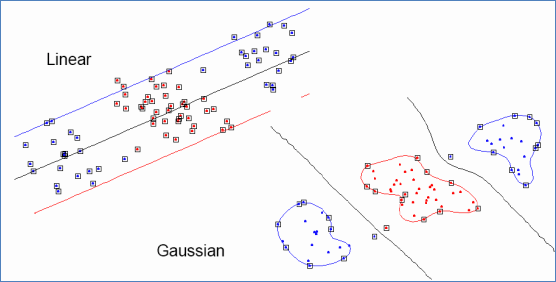
\includegraphics[width=10cm]{kernel_function.png}\\
  \caption {Projection of data from low-dimensional space into higher dimensional space by Radius Basis Function makes inseparable data separable}\label{fig:Fig1}
\end{figure}

\noindent
To be more specific, the Gaussian Process specifies the covariance function as the kernel function which takes the inner dot product between a pair of random variables and we assume the observations have independent identically distributed Gaussian noise, then the prior of the observations becomes:
\begin{equation}\label{eq:14}
  cov(f(x_{a}),f(x_{b})) = k(x_{a},x_{b})+ \sigma_{n}^{2}\delta_{ab}
\end{equation}

\noindent
where the $k(x_{a},x_{b})$ is a general form of kernel function\footnote[{1}]{There are many different kinds of kernel functions such as Radius Basis Function, Polynomial Function and Sigmoid Function. Linear function is also one of the simplest kernel function.} and $\delta_{ab}$ is a Kronecker delta which is one iff $a\equiv b$ and zero otherwise.\\

\noindent
Then, we could generate the joint distribution of the observations $y$ and the predicted value $f_{new}$ under the prior as
\begin{equation}\label{eq:16}
   \left[
    \begin{array}{c}
     y \\ f_{new}
    \end{array}
   \right] \sim N
   \left(
    \begin{array}{cc}
      0 ,& \left[
           \begin{array}{cc}
            k(x,x)+\sigma_{n}^{2}I & k(x,x_{new})\\
            k(x_{new},x) & k(x_{new},x_{new})\\
           \end{array}
          \right]
    \end{array}
   \right)
\end{equation}



\noindent
Deriving the conditional distribution, we finally arrive at the key predictive equations for Gaussian process regression
\begin{align}\label{eq:17}
   f_{new}|x,y,x_{new} &\sim N(\bar f_{new}, cov(f_{new})), \quad where\\
   \bar f_{new} &= k(x_{new},x)[k(x,x)+\sigma_{n}{2}I]^{-1}y\\
   cov(f_{new}) &= k(x_{new},x_{new})-k(x_{new},x)[k(x,x)+\sigma_{n}{2}I]^{-1}k(x,x_{new})
\end{align}

\noindent
This equations give us the corresponding mean value and covariance value of the predictive point which is used to represent the predicted point. A graphical model of Gaussian Process is can be seen in Fig\ref{fig:Fig2}.

\begin{figure}[h!]
  \centering
  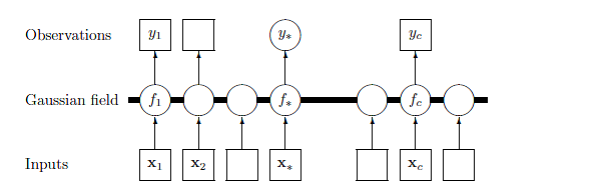
\includegraphics[width=16cm]{GP_model.png}\\
  \caption {Graphical model for a GP for regression.\cite{foo18}}\label{fig:Fig2}
\end{figure}

\section{Multi-Kernel Function}
As mentioned above, the general idea of kernel function is to use it to project the data in low dimensional space to higher one. In general, the kernel function could be divided into two types: global kernel function and local kernel function. The RBF kernel function is considered as typical local kernel while the Polynomial kernel is a global one.\cite{foo21}\\

\noindent
However, both type of kernel function have their own strengths and limitations in different aspects. The local kernel function has strength in terms of approximation but the generalization ability is weak while the global one has stronger generalization ability but weaker approximation capacity.\\

\noindent
We want to take the advantages from the kernel function and eliminate its weakness as much as possible. Therefore, to overcome the weakness of the single kernel function, one simple way is combining those two types of kernel function together as a multi-kernel function, such as the RBF and the Polynomial one.

\begin{equation}\label{eq:222}
  k_{mix} = m*k_{poly} + (1-m)*k_{rbf}  ( 0 \leq m \geq 1)
\end{equation}

\noindent
where $m$ is the weight between two kernel functions. We can see that if $ m = 0$, the multi-kernel is actually a RBF kernel and it is a polynomial kernel when $m = 1$. By combining two kernels as a new one and find a proper weight between them, we could achieve our goal. As for how to find the proper weight factor $m$, we will explain in the section of optimization. The performance of this multi-kernel function will also be evaluated and compared to the single kernel function later.

\section{Property of Gaussian Process}

As a supervised learning algorithm, the Gaussian Process are also based on the idea that similar input give result in the similar outputs or output distributions. But it also have its unique strengths compare with ANN (Backpropagation (BP) algorithm as example) and SVR. \\

\noindent
When it comes to BP algorithm, firstly, Since BP algorithm is based on the Empirical risk minimization, it is minimizing the expected error of the model by minimizing the differences between the output of training data and their corresponding true value. This will lead to a serious overfitting problem and poor generalization for new data since it only optimizes the parameters based on training set without considering the test set. Secondly, for a particular BP model, the number of layers of hidden units and the number of units in each layers play an irreplaceable role in ANN algorithm but how to decide these value still remain as a series problem and need to solved. Besides, the BP model adjusted the weights by iteratively calculating the difference between the predicted value and the true ones and giving feedbacks to the system, this principle is in fact similar to the idea of gradient descending. As a result, it will have a low convergence rate and could not guarantee to find the global optima every time.\\

\noindent
As for the SVR, it improves this situation by using structure risk minimization and introducing the penalty coefficient. The structure risk minimization describes the minimization of the sum of the empirical risk and VC confidence which is caused by the complexity of the function space. These principles could avoid the overfitting problem efficiently and allow the model to have a better generalization capacity. However, the SVR still has many obvious problems such as the choice of the type of kernel function and its parameters and the proper value for the penalty coefficient. In addition, the output of SVR is lack of probabilistic meaning.\\

\noindent
The Gaussian Process is based on the Gaussian distribution and Bayesian theory which implies a solid foundation of probabilistic and statistic. For example, the Gaussian Process not only give the predicted value but also the uncertainty of the prediction. This property makes the prediction easier to interpret and understand. What's more, since Gaussian Process make the prediction based on the distribution of all data and weaken the contribution of single outlier, it prevents the overfitting problem and gives better generalization capacity than SVR. In addition, in terms of the choice of hyperparameters, the Gaussian Process is self-adaptive. In other words, the Gaussian Process choose the optimal hyperparameters during its process of training a model while SVR could only choose them by using cross-validation method or based on the pervious experiences. Besides, compared with the BP and SVR model, the number of parameters of Gaussian Process is quite small which makes the optimization easier to be implemented.\\


\chapter{Feature selection}
\fontsize{12pt}{16pt}\selectfont

Another key point of this thesis is the feature selection. As mentioned in section 2, most of the state-of-art features have strong connection with the biology aspect. However, few of the so-called less-biological meaningful features have been implemented and investigated so far. Therefore, in this chapter, we will introduce some methods of feature selection that the selected features have less biological meaning and explain the theory behind each of them. The performance of these features will be compared with some benchmarks and fully discussed in the chapter 6.\\

\section{Bag of Word}
The idea of feature selection by Bag of Word method is implement comparison of strings by embedding sequential data in a vector space.\cite{foo17}.\\

\noindent
To be more specific, the peptide sequence is characterized by a predefined set of strings which is considered as the embedding language $L$ and each of the strings in this set is the word $w$ of $L$. In general, there are two ways to define the embedding language $L$ and its words $w$. Here we only discuss one method called $n-grams$.\\

\noindent
The $n-grams$ method is simply shift a small window with fixed length $n$ along all of the peptide sequences to extract substrings with length $n$. The language $L$ is then consist of all the possible substrings that have been extracted.\\

\noindent
After establishing the embedding language $L$, we try to project each peptide $p_{i}$ into a vector space composed by the words of $L$ using a function $\phi$
defined as
\begin{equation}\label{eq:18}
  \phi : p_{i} \rightarrow \phi_{w}(p_{i}), \quad w \in L
\end{equation}

\noindent
where the return of $\phi_{w}(p_{i})$ is defined as frequency for the occurrences of $w$ in $p_{i}$.\\

\noindent
In our case, we use $2-grams$ method to build our embedding language $L$ then each $w$ in $L$ is a 2-amino-acid group and since we have 20 different amino acid in total, each of the peptide will be represented by the frequencies of occurrences of 400 words. A graphical flow of the bag-of-word method can be seen as Fig.\ref{fig:Fig5}:

\begin{figure}[h!]
  \centering
  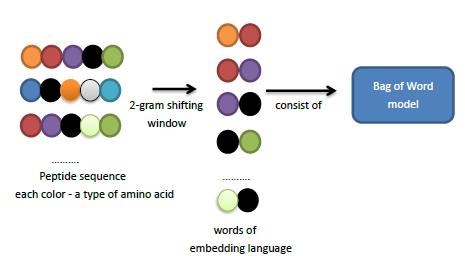
\includegraphics[width=10cm]{BOW.png}\\
  \caption{Bag of Word}\label{fig:Fig5}
\end{figure}

\noindent
Since the number of the words $w$ in $L$ is directly related to the length of the peptide sequence, the length of the peptide will be used as a feature to characterize the peptide.\\

\noindent
In addition, knowing that the hydrophobicity has influenced the retention time of the peptide greatly, it is reasonable to include the hydrophobicity of the peptide in the feature set too.\\

\noindent
The advantages of the Bag-of-Word method are mainly showed in two aspects: complexity and flexibility.\\

\noindent
In terms of complexity, the most popular features that have been used nowadays are biological features. However, in order to calculate these features, a large amount of time is required. What's worse, some particular facilities are needed to calculate some of them, for example, we need to use  the secondary structure. Comparing with these features extraction methods, the computational cost of our method is very low. According to \cite{foo17}, the run-time complexity of Bag-of-Word is $O(|x|+|y|)$ when it is  $O(|x|\cdot |y|)$  for another benchmark method.\\

\noindent
When it comes to the flexibility, since the embedding language $L$ is constituted by the words that are directly and simply extracted from the samples, this method could easily change the language set $L$ for particular context of the task which might imply a wider applicability in other field of biological research.\\


\chapter{Optimization}
\fontsize{12pt}{16pt}\selectfont

In the Gaussian Process model, the most important part is the covariance function of the model since the Gaussian Process consider it as the kernel function. The value of the covariance function along with the value of mean function are known as the hyperparameters in this case. Initially, we need to determine the hyperparameters manually. However, since we do not know the best combination of these hyperparameters beforehand, therefore, we have a group of parameters $[ m, \sigma , \mu]$ where $m$ is the weighted factor of kernel function and $\sigma$ is the value of covariance function and $\mu$ represent the value of mean function that need to be optimized for the best performance.\\

\noindent
As for the definition of optimizing the model, we simply aim at minimizing the error between the predicted retention time and the true one. Thus, the objective function in this case is the negative log marginal likelihood of Gaussian Process as \ref{eq:20}

\begin{equation}\label{eq:20}
  min f(x) =-logp(y|x,\theta)
   =\frac{1}{2}y^{T}(C)^{-1}y+\frac{1}{2}log|C|+\frac{n}{2}log(2\pi)
\end{equation}
where $C =k(x,x)+\sigma_{n}^{2}I_{n}$\\

\noindent
Here, we will implement two different optimization method that based on different principles. The first one is Conjugate Gradient method and the second one is Particle Swarm Optimization method. The principle of each method will be explained in detail along with their own strengths and drawbacks towards this case.

\section{The Conjugate Gradient}

Since we want to optimize the hyperparameter group $[ w, \sigma , \mu]$, we will try to find the minimum value of the objective function. The conjugate gradient method (CG)is one of widely used method and is developed based on the gradient descending method and Newton Method.\\

\noindent
In CG theory, we have two important assumptions:
\begin{itemize}
  \item Linearity:\\
        the $k_{th}$ search direction $d_{k}$ is the linear combination of all the previous directions.
  \item Conjugation:\\
        all the search direction are conjugated with some positive definitive matrix $A$.
\end{itemize}

\noindent
The first assumption allow as to have the follow equation:

\begin{equation}\label{eq:21}
  d^{k} = -g^{k} + \beta_{k-1}d^{k-1}
\end{equation}
where$g^{k+1}$ is the gradient of current point and $\beta_{k}$ is some coefficients that need to be calculated. The second assumption is actually used to allow us calculating the $\beta_{k}$\\

\noindent
The process of Conjugate Gradient(CG) method could be described as Fig.\ref{fig:Fig7}
\begin{figure}[h!]
  \centering
  % Requires \usepackage{graphicx}
  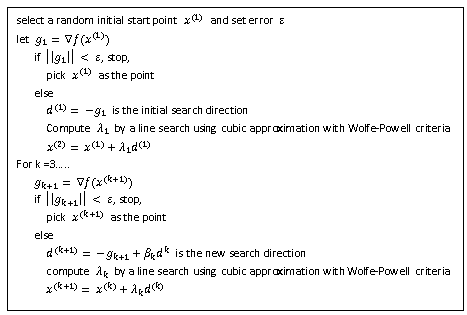
\includegraphics[width=10cm]{CG_algorithm.png}\\
  \caption{Conjugate Gradient algorithm}\label{fig:Fig7}
\end{figure}

\noindent
From the algorithm above, we could see the CG method firstly finds a descent direction along which the objective function \ref{eq:20} will be reduced and then computes a step size that determines how far should we move along the direction, aiming at find a local minimum of the objective function.\\

\noindent
Therefore, the problem could approximately be divided into two parts: Searching the descending direction and determining the step size iteratively. To be more specific, find the proper value for parameters $\beta_{k}$ and $\lambda_{k}$ respectively.\\

\noindent
When it comes to the search direction, due to the second assumption of CG method, we could know that

$$ \beta_{j} =\left\{
\begin{aligned}
  &= 0 \quad j=0....k-1\\
  &\neq 0 \quad j=k
\end{aligned}
\right.
$$

\noindent
Therefore, we are able to compute the $\beta_{k}$ by some methods. In fact, we have many different ways to calculate the parameters $\beta_{k}$ and each of them based on different principles. Here, we implement the Polak-Ribiere method\cite{foo19} that compute the parameter $\beta_{k}$ as \ref{eq:22}.\\

\begin{equation}\label{eq:22}
  \beta_{k} = \frac{g_{k+1}^{T}(g_{k+1}-g_{k})}{g_{k}^{T}g_{k}}
\end{equation}

\noindent
After getting the new search direction $d^{(k+1)}$, the problem comes to define the step size $\lambda_{k}$. Here, we use cubic approximation as \ref{eq:23} to compute the new step size.

\begin{align}\label{eq:23}
   &\lambda_{k} = \lambda_{k-2}-\frac{(-d^{(k-2)}d^{(k-2)})*(\lambda_{k-1}-\lambda_{k-2})^{2}}{(B+\sqrt{(B*B-A*(-d^{(k-2)}d^{(k-2)}))*(\lambda_{k-1}-\lambda_{k-2})})}\notag\\
   &A =6*(f(x_{k-2})-f(x_{k-1}))-3*(-d^{(k-1)}d^{(k-1)}+(-d^{(k-2)}d^{(k-2)}))*(\lambda_{k-1}-\lambda_{k-2})\notag\\
   &B=3*(f(x_{k-1})-f(x_{k-2}))-(2*(-d^{(k-2)}d^{(k-2)})+(-d^{(k-1)}d^{(k-1)}))*(\lambda_{k-1}-\lambda_{k-2})
\end{align}


\noindent
We will then calculate the objective function value $f(x_{k}+a_{k}d_{k})$ and new slope $g_{k+1}^{T}d_{k}$ based on this new step size $\lambda_{k}$ and judge it by using the Wolfe-Powell conditions as \ref{eq:24}

\begin{align}\label{eq:24}
   f(x_{k}+\lambda_{k}d_{k})&\leq f(x_{1})+\lambda_{1} \rho g_{1}^{T}d_{1}\notag\\
   g_{k+1}^{T}d_{k} &\geq \sigma g_{1}^{T}d_{1}  \quad \quad \sigma \in (\rho,1),\quad \rho \in (0,\frac{1}{2})
\end{align}

\noindent
If the current point objective function value and slope fulfill the Wolfe-Powell conditions, we could claim we find the proper step size that is calculated by the cubic extrapolation and stop searching.\\

\noindent
By doing these iteratively, we could minimize the objective function and eventually have the set of hyperparameters $[ w, \sigma , \mu]$ that gives the minimum value of the objective function or fulfills the required accuracy.

\noindent
The CG method is based on the gradient descent and Newton method. It only uses the information provided by the first order derivative which means it does not need any further information and could be easily implemented in many aspects. \\

\noindent
This property also implies that it does not need to compute and store the Hesse Matrix as well as its inverse. As a result, it could reduce the computational cost significantly compared with the Newton method.\\

\noindent
What's more, since the traditional gradient descent method will slow down the searching rate dramatically when it is getting closer to the minimal value, the CG manage to overcome this drawback of the gradient descent by using the conjugation which could speed up the convergence rate. The following plots show the convergence rate of two different methods\\


\begin{figure}[h!]
\centering
\subfigure[Gradient Descent]{
\label{Fig.sub.1}
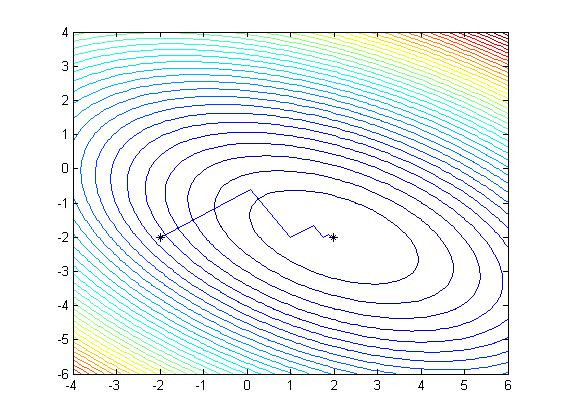
\includegraphics[width=0.4\textwidth]{Gradient_Descent.jpg}}
\subfigure[Conjugate Gradient]{
\label{fig:sub1}
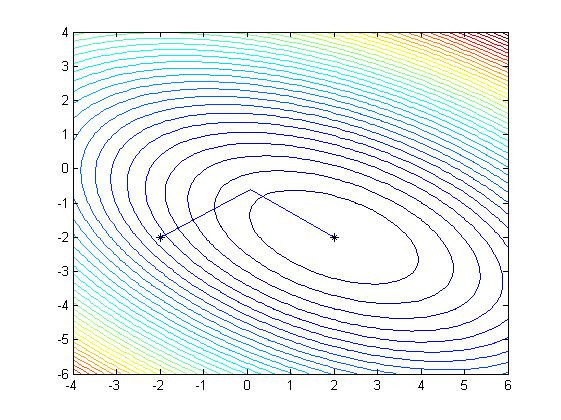
\includegraphics[width=0.4\textwidth]{CG.jpg}}
\caption{Comparison of convergence rate}
\label{fig:sub2}
\end{figure}


\section{The Particle Swarm Optimization}

The Particle Swarm Optimization (PSO) method is one of the new iterative methods for problem optimization. It improves the solution by iteratively searching for the best result in current circumstance. \\

\noindent
Initially, we have a branch of separated particles that represent the potential solution by their position, a group of parameters $[ w, \sigma , \mu]$ in our case. And for each parameter in the one particle, we assign different velocity for them. In each iteration, the particle updates its position simply by its velocity of each parameter. Then we using these parameter to calculate the model and evaluate the result by some predefined loss functions. After that, we record the best position for each particle(local optimal value) as well as the best position in the whole search space(global optimal value).\\

\noindent
The smart part of this method is the update of the velocity of each particle. The individual velocity for each particle is influenced not only by its local best known position (local optimal value) but also the best known positions in the search-space (global optimal value), which are updated as better positions are found by other particles. This is expected to move the swarm toward the best solution.\\

\noindent
In the end, the iteration will be terminated by some criterion, such as the maximal number of iterations or a solution that gives the adequate loss function value is found. The following Fig. \ref{fig:Fig8} shows the basic algorithm of Particle Swarm Optimization \\

\begin{figure}[h!]
  \centering
  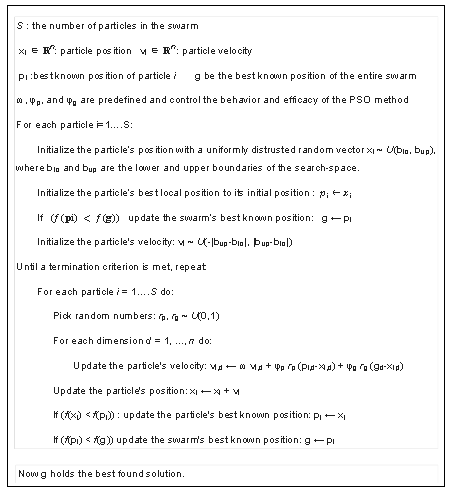
\includegraphics[width=12cm]{PSO.png}\\
  \caption{Particle Swarm Optimization}\label{fig:Fig8}
\end{figure}

\noindent
PSO is a heuristic search algorithm based on swarm intelligence since it makes no assumptions about the problem being optimized and can search very large spaces. Therefore, PSO can also be used on optimization problems that are partially irregular, noisy, change over time, etc. What's more, since it uses swarm intelligence which means each of the particle is related to the others and the final result is depended on the contribution of all particles, the robustness of system is strong and will not be be dramatically influenced by some outliers. In addition, its strengths in terms of convergence, global search capacity and practicability also make it one of the most popular optimization algorithm in the world. \\


\chapter{Results and Evaluation}
\fontsize{12pt}{16pt}\selectfont

In this section, we report the experiments in order to compare the GP regression model with other regression model and discuss their performance. We are interested in whether the GP model leads to a better predictive performance. \\

\noindent
To get a better impression of the performance, we will firstly compare the GP model with single kernel to the one with multiple kernels. Further, we will report the performance of $\epsilon-SVR$ using an RBF kernel as an benchmark to the GP model. This $\epsilon-SVR$ model is based on the loss function

\begin{equation}\label{eq:25}
  \centering
  |y_{i} - f(x_{i})|_{\epsilon} = max\{0 , |y_{i} - f(x_{i})|-\epsilon\}
\end{equation}

\noindent
which is summed over all $i =1,.....,N$ training data. The RBF kernel used in SVR model is similar to the RBF kernel in GP covariance function.  However, this is a clear disadvantage compared to the parameterisations we implemented in the GP models because the scaling of input variables becomes a sensitive issue.\\

\noindent
After comparing the GP model with the SVR model, we will investigate the importance of optimization. In another word, we will compare the results before and after optimization for both GP model and SVR model respectively. In the end, we will evaluate the performance of different optimization methods, PSO and CG method specifically. All these model will be tested in two different set of features respectively so that we could make a comparison between different kind of features. The first kind of feature is the feature created by Bag of Word method: we simply call it $BOW feature$, and the second one is the feature used for prediction in the state-of-art model Elude: we call it $Elude feature$.\cite{foo5}\\

\noindent
Before introducing the experimental setup, we will introduce two main concepts which we will use for evaluation later: Pearson Correlation Coefficient and minimal time window.
\begin{itemize}
  \item Pearson Correlation Coefficient:\\
        In statistic theory, Pearson correlation coefficient is used to identify the linear correlation between two variables $X$ and $Y$. The formula is as follow:
\begin{equation}\label{eq:25}
   \rho = Cor(X, Y) = \frac{Cov(X,Y)}{\sqrt{Var(X)Var(Y)}}
\end{equation}
        The value of Pearson Correlation Coefficient is between -1 and 1. A value of 1 (or -1)implies that a linear equation describes the relationship between X and Y perfectly, the sign implies whether the relationship is positive or negative. A value of 0 implies that there is no linear correlation between the variables. The closer the value is to 1, the stronger the linear relation they have, otherwise, the weaker the relation they have.\\
  \item Minimal Time Window:\\
        The minimal time window is a time window including the
        deviations between observed and predicted retention times for
        95\% of the peptides ($\Delta t95\%$). Given the time window, we could know the expected range of observing time in advance and thus enhanced paralleling generating ability of the retention time of peptide. In this case, the minimal time window will be showed as ratio of total time instead of a absolute value. The smaller the time window is, the more peptide we could generating at the same time.

\end{itemize}

\noindent
In this thesis, the top priority is given to minimize the minimal time window since we want to be able to generate peptide as many as possible and improve the parallelized processing capacity. Therefore, even if the Pearson coefficient coefficient of model A is sightly better than model B, we still claim the model B has better performance than A when the minimal time window of model B is smaller than A.

\section{Experimental Setup}
The experiment is tested on a 64-bit Ubuntu computer and run by Matlab R2014a. To build the Gaussian Process model, we need to install the software package called GPML which is written by Carl Edward Rasmussen and Hannes Nickisch.\cite{foo18} In addition, to benchmark the GP model, we also need the SVR software packages include libsvm \cite{foo20}.
\section{Experimental result}

\begin{figure}[h]
\centering
\subfigure[Bag of Word feature with RBF kernel]{
\label{Fig.sub.1}
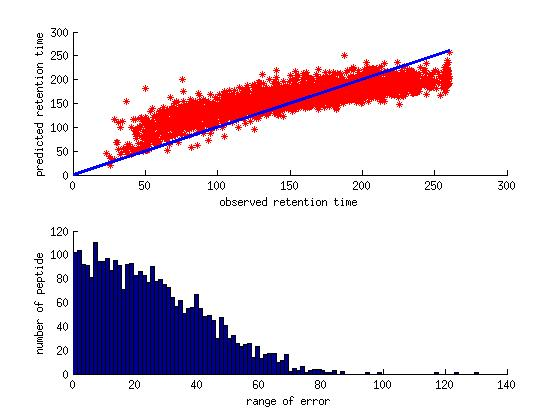
\includegraphics[width=0.4\textwidth]{original_without_opt_usingbow.jpg}}
\subfigure[Bag of Word feature with RBF+Poly kernel]{
\label{Fig.sub.2}
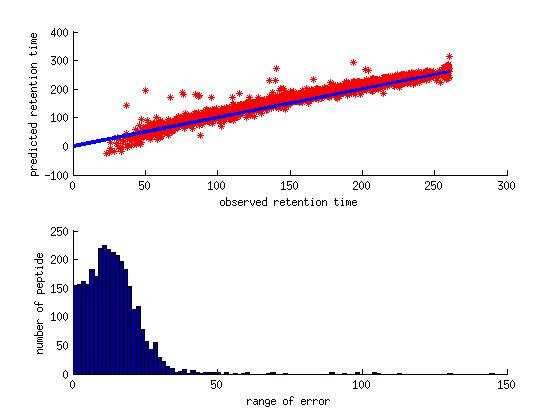
\includegraphics[width=0.4\textwidth]{original_without_opt_bowfeature_multikernel.jpg}}
\caption{Comparison of performance based on different kernels} \label{fig:Fig9}
\end{figure}

\noindent
The Gaussian Process model is firstly built by $BOW feature$. The Fig.\ref{fig:Fig9} shows the performance of the GP model based on different kernel function. The left one is simply using RBF kernel while the right one is using a multiple kernel that consist of RBF and Poly kernel function. The blue line in the plot represents the ideal result of the correlation coefficient and the red one is the true results from the experiment.\\

\noindent
For each subplot, the top plot shows the correlation between the predicted retention time and the real retention time and tells how linear they are related to each other. The histogram in the bottom shows the the distribution of the deviation between the predicted retention time and the real one. \\

\noindent
As benchmark, we also test the model by using $Elude feature$. The fig.\ref{fig:Fig10} gives us the performance of the model based on this feature set.\\

\begin{figure}[h]
\centering
\subfigure[Elude feature with RBF kernel]{
\label{fig:sub1}
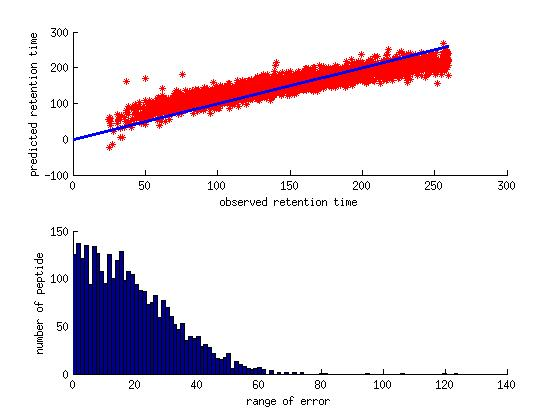
\includegraphics[width=0.4\textwidth]{original_without_opt.jpg}}
\subfigure[Elude feature with RBF+Poly kernel]{
\label{Fig.sub.2}
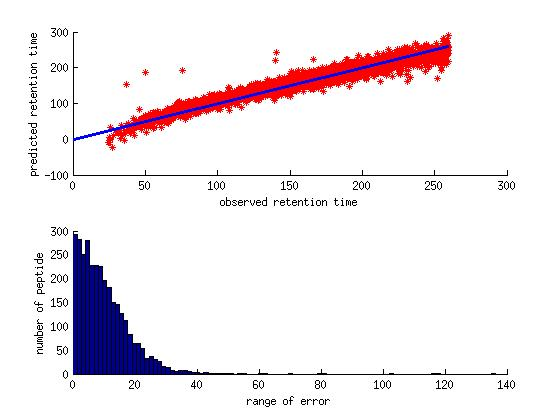
\includegraphics[width=0.4\textwidth]{Lumi_RBF+poly_without_opt_GP.jpg}}
\caption{Comparison of performance based on different kernel with Luminita's feature}
\label{fig:Fig10}
\end{figure}

\noindent
The Table.\ref{table1} shows detail information in terms of the Pearson Correlation Coefficient and the minimal time window of them. The left number is the Person Coefficient and the right one is the corresponding minimal time window.\\

\begin{table}[h]
\normalsize
\centering
%\begin{tabular}{m{3cm}|m{3cm}|m{3cm}}
\begin{tabular}{l|cc|cc}
         & \multicolumn{2}{c|}{RBF kernel} & \multicolumn{2}{c}{RBF + Poly kernel}\\
         & $\rho$ & $\Delta_{t95\%}$ & $\rho$ & $\Delta_{t95\%}$ \\      
        \hline
         BOW feature & 0.8508 & 0.4191 &  0.9724 &  0.1822\\
        \hline
         Elude feature  & 0.9213 & 0.3346 &  0.9683 & 0.1718\\
        \hline
\end{tabular}
\caption{Comparison between Single kernel and multi-kernel}
\label{table1}
\end{table}

\noindent
As we can see from the figures, the multi-kernel gives better performance than a single kernel in general. The multi-kernel function helps GP model to improve the correlation coefficient as well as reduce the minimal time window dramatically, from 0.4191 to 0.1822 and 0.3346 to 0.1718 for $BOW feature$ and $Elude feature$ respectively. \\

\noindent
After comparing the Gaussian Process with single kernel and multi-kernel, we would like to compare the Gaussian Process model with the traditional Support Vector Regression model and investigate the performance. Since we already known the multi-kernel gives better performance, we will only use the Gaussian Process model with multi-kernel for all the GP model later.\\

\begin{figure}[h!]
\centering
\subfigure[BOW feature with SVR model]{
\label{fig:sub1}
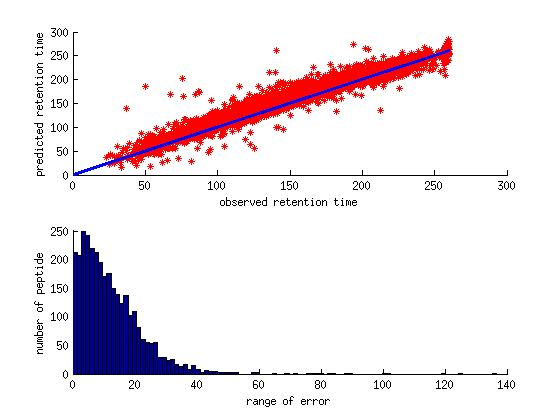
\includegraphics[width=0.4\textwidth]{bow_svr_without_opt.jpg}}
\subfigure[Elude feature with SVR model]{
\label{Fig.sub.2}
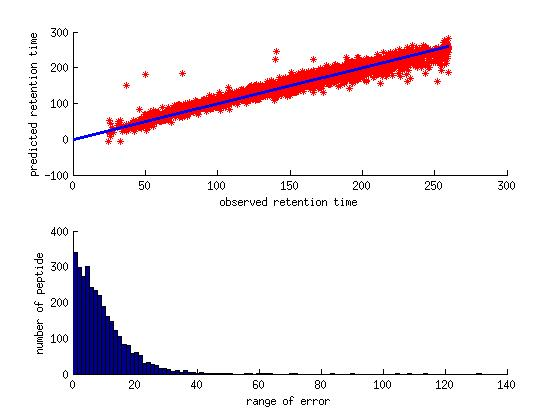
\includegraphics[width=0.4\textwidth]{Lumi_svr_without_opt.jpg}}
\caption{Performance of the feature based on Support Vector Regression model}
\label{fig:Fig12}
\end{figure}

\noindent
The fig.\ref{fig:Fig12} gives us the visual performance of SVR model. Although the difference is hard to tell from this plot, we will summarize its performance and make the comparison in Table.\ref{table2}.

\begin{table}[h]
\normalsize
\centering
\begin{tabular}{m{2.5cm}|m{5cm}|m{5cm}}
        \hline
                & Gaussian Process ( RBF+Poly ) & Support Vector Regression\\
        \hline
         BOW feature & 0.9724 \quad 0.1822 &  0.9655 \quad 0.2095\\
        \hline
         Elude feature  & 0.9683 \quad 0.1718 &  0.9701 \quad 0.1809\\
        \hline
\end{tabular}
\caption{Comparison of performance between GP (multi-kernel) and SVR model}
\label{table2}
\end{table}

\noindent
As we can see from the Table.\ref{table2}, the $\epsilon-SVR$ model gives a bit better performance in terms of the correlation coefficient when predicting the retention time by Elude features. However, the $\epsilon-SVR$ model gives worse results in terms of minimal time window in both cases. Therefore, the GP model is better than the $\epsilon-SVR$ in this case.\\

\noindent
After comparing the GP and SVR model without optimization, we will now investigate the effect of optimization. In this case, we only perform two models with Particle Swarm Optimization method as an example. The following plots show the results

\begin{figure}[h!]
\centering
\subfigure[BOW feature with SVR model]{
\label{fig:sub1}
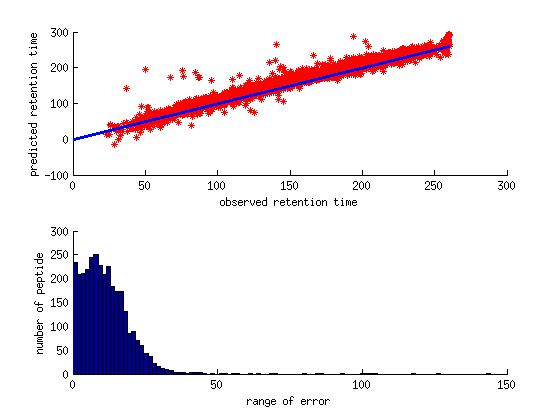
\includegraphics[width=0.4\textwidth]{PSO_fig2_bow_svr.jpg}}
\subfigure[Elude feature with SVR model]{
\label{Fig.sub.2}
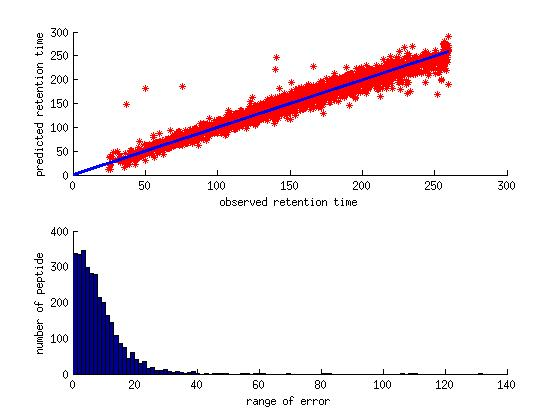
\includegraphics[width=0.4\textwidth]{Lumi_svr_PSO_fig2.jpg}}
\caption{Performance of the feature based on Support Vector Regression model after PSO optimization}
\label{fig:Fig13}
\end{figure}

\begin{figure}[h!]
\centering
\subfigure[BOW feature with GP model]{
\label{fig:sub1}
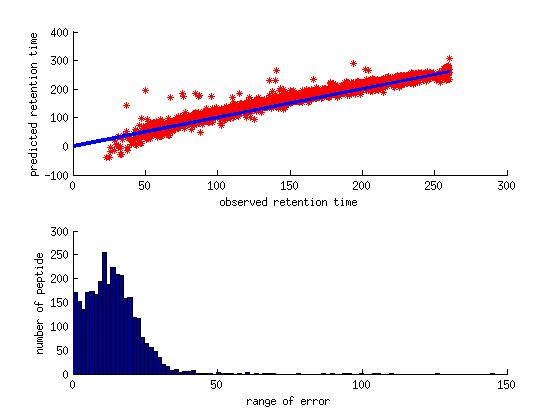
\includegraphics[width=0.4\textwidth]{PSO_fig1_bow.jpg}}
\subfigure[Elude feature with GP model]{
\label{Fig.sub.2}
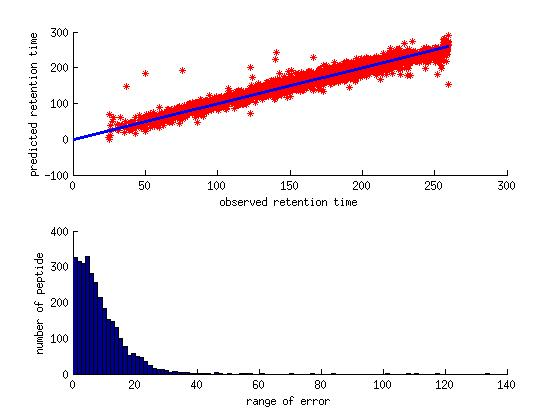
\includegraphics[width=0.4\textwidth]{PSO_fig1_Lumi.jpg}}
\caption{Performance of the feature based on Gaussian Process model after PSO optimization}
\label{fig:Fig14}
\end{figure}

\begin{table}[h]
\normalsize
\centering
\begin{tabular}{p{1cm}|p{2cm}|p{3.5cm}|p{3.5cm}}
\hline
\multicolumn{2}{c|}{} & Before Optimization & After Optimization \\
\hline
\multirow{2}{*}{GP} & BOW  & 0.9734 \quad 0.1822 & 0.9751 \quad 0.1731 \\
\cline{2-4}
 & Elude & 0.9683 \quad 0.1718 & 0.9741 \quad 0.1537 \\
\hline
\multirow{2}{*}{SVR} & BOW  & 0.9655 \quad 0.2095 & 0.9744 \quad 0.1628 \\
\cline{2-4}
 & Elude & 0.9701 \quad 0.1809 & 0.9762 \quad 0.1537 \\
\hline
\end{tabular}
\caption{Comparison of performance before and after PSO for GP and SVR model}
\label{table3}
\end{table}

\noindent
From Table.\ref{table3}, we could tell that the optimization plays a irreplaceable role in our prediction. The optimization helps to reduce almost 5\% of the minimal time window. This therefore could allow more peptide to be generated in the same time and enhance the parallelized processing capacity in a dramatic way.\\

\noindent
We could also see that the general performance of $\epsilon-SVR$ is slightly better than the GP model after optimization. However, the time consumption becomes a serious problem in this case. For example, the running time for $\epsilon-SVR$ based on $Elude feature$ is $101742 sec$ while the time for GP model based on the same feature is only $3869 sec $. Considering the top priority for the prediction is to improve the parallelized processing capacity (minimal time window) while maintain acceptable accuracy, the GP model is still better than the $\epsilon-SVR$.\\

\noindent
Now we will try to make a comparison of different optimization methods, PSO and CG method specifically. In this case, we will only use the GP model as example since it gives better performance than the $\epsilon-SVR$ in general. The following plots show the experimental results.

\begin{figure}[h!]
\centering
\subfigure[BOW feature with PSO]{
\label{fig:sub1}
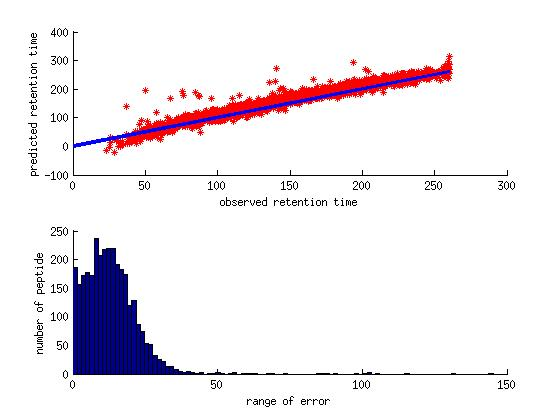
\includegraphics[width=0.4\textwidth]{PSO_fig1_BOW_mk.jpg}}
\subfigure[BOW feature with CG]{
\label{Fig.sub.2}
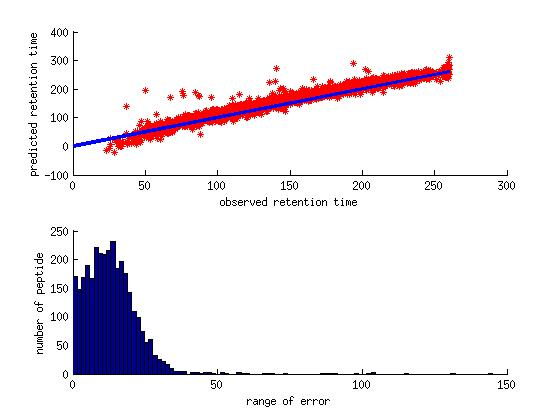
\includegraphics[width=0.4\textwidth]{CG_fig1_BOW_50times_iter.jpg}}
\caption{Performance of the BOW feature based on different optimization method}
\label{fig:Fig15}
\end{figure}

\begin{figure}[h!]
\centering
\subfigure[Elude feature with PSO]{
\label{fig:sub1}
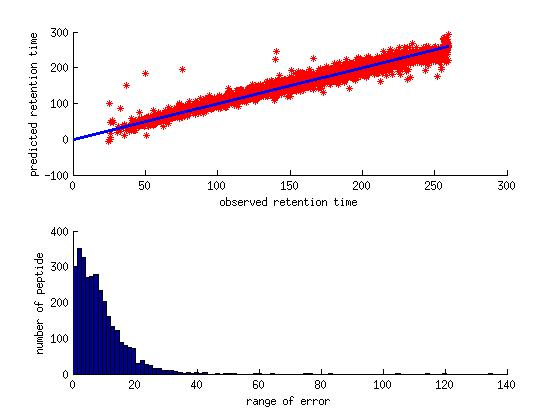
\includegraphics[width=0.4\textwidth]{PSO_fig1_Lumi_mk.jpg}}
\subfigure[Elude feature with CG]{
\label{Fig.sub.2}
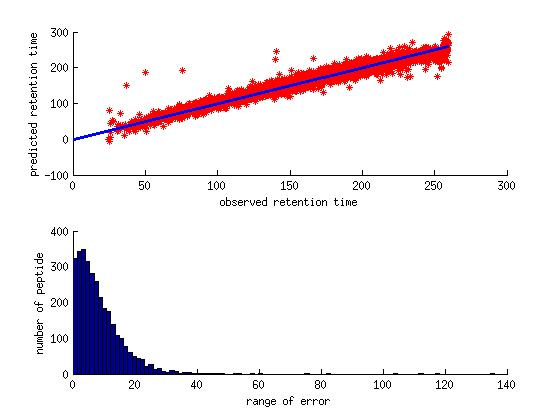
\includegraphics[width=0.4\textwidth]{CG_fig1_Lumi_50times_iter.jpg}}
\caption{Performance of the Elude feature based on different optimization method}
\label{fig:Fig16}
\end{figure}


\noindent
The details of the comparison of these two optimization method are summarized in Table.\ref{table4} below. As we can see, these two methods have similar performance in this case. However, this is not always the case and the reasons why this happen will be explained and discussed in the next chapter.\\

\begin{table}[h!]
\normalsize
\centering
\begin{tabular}{p{1cm}|p{4.5cm}|p{3.5cm}}
\hline
   & Particle Swarm Optimization & Conjugate Gradient \\
\hline
 BOW  & 0.9751 \quad 0.1731 & 0.9744 \quad 0.1731 \\
\hline
 Elude & 0.9744 \quad 0.1537 & 0.9757 \quad 0.1537 \\
\hline
\end{tabular}
\caption{Comparison of performance before and after PSO for GP and SVR model}
\label{table4}
\end{table}

\noindent
About the optimization method, apart from having a impression of the general performance, we would also like to investigate the influence of some parameters for the prediction, such as the number of evaluating function, the number of generation, the number of particles and the changing trend of each particle during the evolution.\\

\begin{figure}[h!]
\centering
\subfigure[BOW feature with CG]{
\label{fig:sub1}
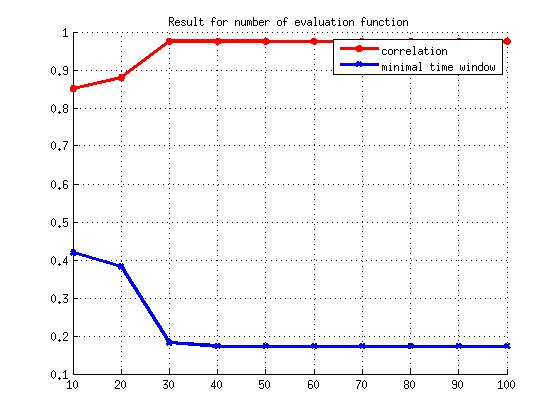
\includegraphics[width=0.4\textwidth]{CG_fig2_bow_cp.jpg}}
\subfigure[Elude feature with CG]{
\label{Fig.sub.2}
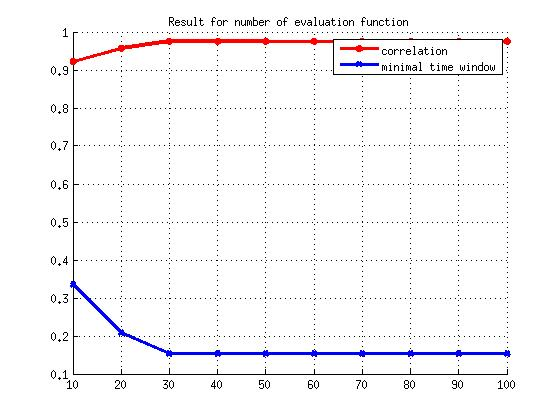
\includegraphics[width=0.4\textwidth]{CG_fig2_lumi_cp.jpg}}
\caption{Comparison of different number of evaluating functions}
\label{fig:Fig17}
\end{figure}

\noindent
The fig.\ref{fig:Fig17} show the effect of different number of evaluating function in CG method based on different features. As we can see, increasing the number of evaluating function results in better performance in terms of correlation coefficient and minimal time window. However, when the number of evaluating function reaches to the level of 30 and above, the difference becomes small and can be ignored. These plots implies that we could set the number of evaluating function around 30 and no need to worry about not getting better prediction result. \\

\noindent
Following this, we will now try to find out the influence of the number of generation in PSO methods.\\

\begin{figure}[h!]
\centering
\subfigure[BOW feature with 5 generation]{
\label{fig:sub1}
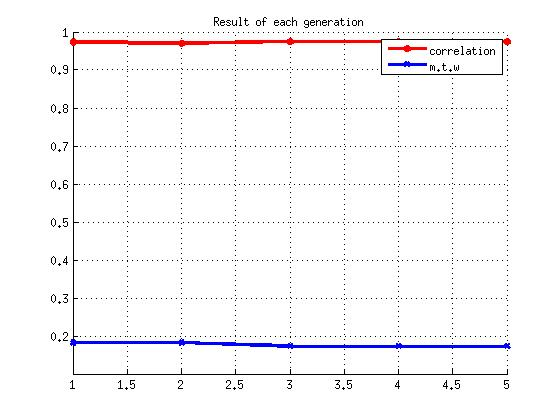
\includegraphics[width=0.5\textwidth]{PSO_bow_5generation.jpg}}
\subfigure[BOW feature with 30 generation]{
\label{Fig.sub.2}
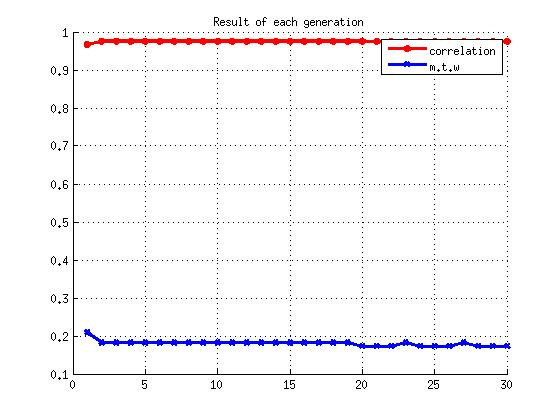
\includegraphics[width=0.5\textwidth]{PSO_fig2_BOW_mk_30generation.jpg}}
\caption{Comparison of different number of generation}
\label{fig:Fig18}
\end{figure}

\noindent
The fig.\ref{fig:Fig18} above shows that the number of generation actually haves slightly influence on the prediction. The top one traces the changing trend of correlation coefficient and minimal time window during 5 generation and in the bottom one, we increase the number of generation to 30 to make a comparison. Each dot in the plots represent the prediction result of that generation.

\begin{figure}[h!]
\centering
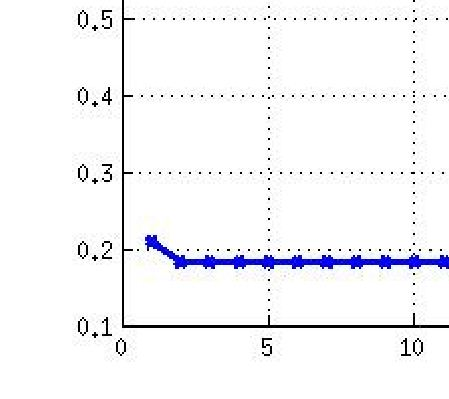
\includegraphics[width=0.5\textwidth]{zoom_in_30generation.jpg}
\caption{Detail changes of 30 generation}
\label{fig:Fig19}
\end{figure}

\noindent
The detail could be seen from fig.\ref{fig:Fig19} that the optimization has reduced the minimal time window from 22\% to around 17\% in the second generation of evolution. Due to the fact that the initial prediction is already really good, the impact of increasing the number of generation seems to be ignorable. Therefore, we could simply set the default number of generation around 5.\\

\noindent
In the end, we will take a look at the effect of different number of particles and each particle's changing trend in terms of correlation coefficient and minimal time window during each generation.\\

\begin{figure}[h!]
\centering
\subfigure[Effect of different number of particle]{
\label{fig:sub1}
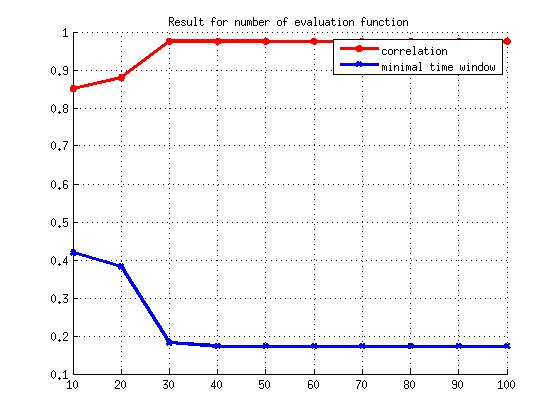
\includegraphics[width=0.5\textwidth]{CG_fig2_bow_cp.jpg}}
\subfigure[Trend of correlation coefficient of each particle]{
\label{Fig.sub.2}
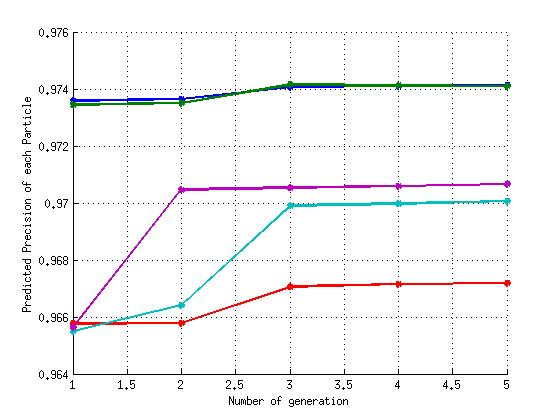
\includegraphics[width=0.5\textwidth]{changing_trend_of_coef.jpg}}
\subfigure[Trend of minimal time window of each particle ]{
\label{Fig.sub.3}
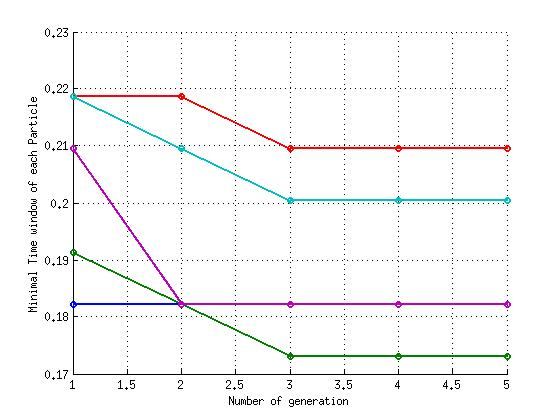
\includegraphics[width=0.5\textwidth]{changing_trend_of_minimal_time_window.jpg}}
\caption{Effect of different number of particles and their changing trend in 5 generations }
\label{fig:Fig20}
\end{figure}

\noindent
As the Fig.\ref{Fig.sub.2} and Fig.\ref{Fig.sub.3} showed, the trend of all the particles in both cases are going towards the better situation and have influenced each other which totally follows the principle of PSO method. One interesting thing is that we could also see the trend becomes more flat and stable after the third generation. This is also support evidence for the conclusion we draw form Fig.\ref{fig:Fig1} about the proper number of generation.


\chapter{Limitation and Discussion}
\fontsize{12pt}{16pt}\selectfont

As we could see from the previous section, the GP model has a better performance in general. However, there are still some limitations of the model that needs to be improved. In this section, we will discuss the limitations in terms of model,feature and optimization methods.

\section{Model limitation}

\noindent
One of the main limitation is the computational cost of Gaussian Process model. Due to the fact that the Gaussian Process Regression model is non-parametric model, for training part, the hyperparameters are obtained by optimizing the margin likelihood function. Therefore, we need to compute the inverse of covariance function $K_{n} + \sigma_{n}^{2}I_{n}$  which makes the computational cost of the model to a level of  $O(n^{3}*p)$ where $p$ is the times of gradient computation. As for the prediction part, the computational cost for each data is $O(n^{2})$. When dealing a large amount of data, this drawback could become more serious and do harm to the implementation.\\

\noindent
Another limitation of the GP model is the assumption of the $Gaussian Noise$ which means the noise fulfills the Gaussian distribution. This assumption makes the GP model easier when calculating the matrix. However, the noise is actually not a $Gaussian Noise$ in some cases and this assumption will influence the prediction.\\


\section{Feature limitation}

As for the features, the main limitation is the lack of information for the features. This limitation is reflected by the fact that the $Elude feature$ performs better than the $BOW feature$ in general.\\

\noindent
However, the accuracy of the prediction and the computational efficiency is a trade-off. On one hand, providing features with less information means the prediction could have more opportunity to be less precisely. On the other hand, compared to those features with more information, these features require less time to be calculated and therefore easier to implemented.\\

\noindent
Since one of the purpose of this thesis to test some less-biology features and investigate their performance, this limitation is unavoidable. Besides, the prediction result of $BOW features$ is still acceptable and not much worse than the one of $ Elude features$.  In addition, considering one of the limitation of GP Model itself is the computational cost, this will compensate the situation.\\

\section{Optimization limitation}

\noindent
Like most evolutionary algorithms, PSO usually requires a large number of fitness evaluations to obtain a sufficiently good solution. This poses an obstacle for applying PSO to computationally expensive problems.\\

\noindent
Besides, as all other heuristic algorithms, PSO do not guarantee an optimal solution is ever found. In fact, the optimized result could be slightly different from time to time but always has the same trend. More specifically, PSO does not use the gradient of the problem being optimized, which means PSO does not require that the optimization problem be differentiable as is required by classic optimization methods such as gradient descent and quasi-newton methods. As a result, it might find the local optimal value instead of the optimal value in the whole search space and consider it as the "global optimal value" due to the its convergence. \\

\noindent
To overcome the shortages of the PSO method, a number of different methods based on the original PSO have been carried out, such as Gray-PSO, Chaos-PSO. Each of these method has combined PSO with some other method so that it could overcome the problem of the original PSO and has its own advantage when dealing with some specific tasks. \\

\noindent
As for the CG method, one of the most limitation of the CG method is its dependency on the initial point which would have a great influence on the final result.Due to this limitation, the CG method could not ensure to converge to the minimum value in the whole search space.\\

\noindent
To overcome this, there are many other CG methods have been carried out. They could improve the performance of the original CG method when dealing with some specific tasks but they still have their drawbacks as well. Since the priority of this thesis is not given to the optimization part, we just simply implement the original methods.\\


\chapter{Conclusion and Future Work}
\fontsize{12pt}{16pt}\selectfont

\section{Conclusion}
In this thesis, a Gaussian Process Regression Model for the prediction of peptide retention time has been proposed and tested in different datasets. Compared with the SVR and ANN methods, the Gaussian Process has better performance in terms of the minimal time window and  computational efficient. By that I mean when having the similar prediction accuracy, the GP model has stronger capacity than SVR and ANN in terms of parallelized processing.\\

\noindent
In addition, a new method of feature selection has been tested in this case. The feasibility of these features has been proved and their performance is as good as the biological features. Although the performance of these features are still slightly worse than the biological features due to the fact of lacking information, the efficiency of generating them and the flexibility of these features still imply the unique advantages of these features.\\

\noindent
In the end, two optimization methods have been implemented and compared with each other. Their properties and the some potential solution of their drawbacks have been discussed too. Besides, the effect of some default parameters of these methods have also been investigated and analyzed .


\section{Future Work}

As we have been analyzing before, one of the most important limitation of GP model is the computational cost. It is quite hard to overcome this problem since the Gaussian Process is non-parametric model. In the last 20 years, many new methods have been carried out to solve this problem. Tresp in \cite{foo22} proposes a Bayesian committee machine(BCM) method and Snelson in \cite{foo23} suggest a method based on sparse Gaussian Process using pseudo-input to enhance the computational efficiency. Therefore, one potential work in the future is to replace the original Gaussian Process with these methods to investigate their performance.\\

\noindent
Another interesting thing is about finding some more proper optimization method to overcome the shortages of current ones. Since we know that the original CG method has the weakness in terms of its dependency of the initial value and the Particle Swarm Optimization could not ensure the convergence to the minimal value of the entire search space, we could try to investigate some new optimization methods which could overcome these drawbacks.\\

\noindent
As one of the newest machine learning method, the Gaussian Process has many strengths when dealing with the problem. However, the theory of Gaussian Process is not complete yet and there are still a lot of aspects need to be fixed and improved. What's more, the application of Gaussian Process method in biotechnological field is still not as common as it is in the other field, such as artificial intelligence or computer vision. Thus, we strongly believe that with the further understanding of Bayesian theory and statistical learning theory as well as the rapidly development of computing techniques, more sophisticated and practical Gaussian Process Regression methods will continually broaden their application fields in biotechnology and new applications, new requirements will lead to continue to the improvement of GP method as well.

 

\begin{thebibliography}{99}

    \bibitem{foo1} Baczek T, Wiczling P, Marszall M, et al. (2005). "Prediction of peptide retention at different HPLC conditions from multiple linear regression models." Journal of Proteome Research, 4(2):555�C63

    \bibitem{foo2} Petritis K, Kangas LJ, Ferguson PL, et al. (2003). "Use of artificial neural networks for the accurate prediction of peptide liquid chromatography elution times in proteome analyses." Analytical Chemistry, 75(5):1039�C48

    \bibitem{foo3}Petritis K, Kangas LJ, Yan B, et al. (2006). "Improved peptide elution time prediction for reversed-phase liquid chromatography-MS by incorporating peptide sequence information." Analytical Chemistry, 78(14):5026�C39.

    \bibitem{foo4}Klammer AA, Yi X, MacCoss MJ, et al. (2007). "Improving tandem mass spectrum identification using peptide retention time prediction across diverse chromatography conditions." Analytical Chemistry, 79(16):6111�C8

    \bibitem{foo5}Luminita Moruz, Daniela Tomazela, Lukas Kall,(2010). "Training, Selection, and Robust Calibration of Retention Time Models for Targeted Proteomics"

    \bibitem{foo6}Luminita Moruz,(2013). "Chromatographic retention time prediction and its applications in mass spectrometry-based proteomics".

    \bibitem{foo7}Mant, C. T., and Hodges, R. S. (2002). "Analytical HPLC of peptides, in HPLC of Biological Macromolecules" (Gooding, K. M., and Regnier, F. E., eds) pp. 433�C511, Marcel Dekker, New York.

    \bibitem{foo8}Meek JL (1980). "Prediction of peptide retention times in high-pressure liquid chromatography on the basis of amino acid composition." Proceedings of the National Academy of Sciences of the United States of America, 77(3):1632�C6.

    \bibitem{foo9}Houghten RA and DeGraw ST (1987). "Effect of positional environmental domains on the variation of high-performance liquid chromatographic peptide retention coefficients." Journal of Chromatography, 386:223�C8.

    \bibitem{foo10}Browne CA, Bennett HP, and Solomon S (1982). "The isolation of peptides by high-performance liquid chromatography using predicted elution positions." Analytical Biochemistry, 124(1):201�C8.

    \bibitem{foo11}Zhou NE, Mant CT, and Hodges RS (1990). "Effect of preferred binding domains on peptide retention behavior in reversed-phase chromatography: amphipathic alpha-helices." Peptide Research, 3(1):8�C20.

    \bibitem{foo12}Mant CT and Hodges RS (2006). "Context-dependent effects on the hydrophilicity/hydrophobicity of side-chains during reversed-phase high-performance liquid chromatography: implications for prediction of peptide retention behaviour." Journal of Chromatography A, 1125(2):211�C9.

    \bibitem{foo13}Guo DC, Mant CT, and Hodges RS (1987). "Effects of ion-pairing reagents on the prediction of peptide retention in reversed-phase high-performance liquid chromatography." Journal of Chromatography,386:205�C22.

    \bibitem{foo14}Gilar M, Xie H, and Jaworski A (2010). "Utility of retention prediction model for investigation of peptide separation selectivity in reversed-phase liquid chromatography: impact of concentration of trifluoroacetic acid, column temperature, gradient slope and type of stationary phase." Analytical Chemistry, 82(1):265�C75.

    \bibitem{foo15}Krokhin OV, Craig R, Spicer V, et al. (2004). "An improved model for prediction of retention times of tryptic peptides in ion pair reversed-phase HPLC:its application to protein peptide mapping by off-line HPLC-MALDI MS." Molecular Cellular Proteomics, 3(9):908�C19.

    \bibitem{foo16}Kaliszan R, Baczek T, Cimochowska A, et al. (2005). "Prediction of high-performance liquid chromatography retention of peptides with the use of quantitative structure-retention relationships." Proteomics, 5(2):409�C15.

    \bibitem{foo17}Konrad Rieck.(2011)"Similarity measures for Sequential data"

    \bibitem{foo18}C. E. Rasmussen C. K. I. Williams,(2006) "Gaussian Processes for Machine Learning", the MIT Press.

    \bibitem{foo19}B. T. Polyak. (1969) "The conjugate gradient method in extreme problems." USSR Comp Math Math Phys, 9(4): 94-112.

    \bibitem{foo20}Chang CC and Lin CJ (2011). LIBSVM: A library for support vector machines. ACM Transactions on Intelligent Systems and Technology, 2:27:1�C27:27. Software available at http://www.csie.ntu.edu.tw/~cjlin/libsvm.

    \bibitem{foo21}S Zhang, J liu, J.W Tian(2004) An SVM-based small target segmentation and clustering approach [C].In: Proceedings of the Third International Conference on Machine Learning and Cvbernetics.Shanghai:IEEE,2004,6(8):3318-3323.
    
    \bibitem{foo22} Tresp V. A Bayesian committee machine[J]. Neural
        Computation, 2000, 12: 2719-2741.
     
    \bibitem{foo23}Snelson E, Ghahramani Z. Sparse Gaussian processes
        using pseudo-inputs[C]. Proc of the NIPS 18. Vancouver, 2006: 1257-1264



\end{thebibliography}

.
\end{document}
